\documentclass[11pt]{article}
\usepackage[utf8]{inputenc}
\usepackage{amsmath,amssymb}
\usepackage{graphicx}
\usepackage{hyperref}
\usepackage{geometry}
\usepackage{booktabs}
\usepackage{enumitem}
\usepackage{listings}
\usepackage{xcolor}
\usepackage{longtable}
\usepackage{multirow}
\geometry{margin=1in}

\lstset{
    basicstyle=\ttfamily\footnotesize,
    breaklines=true,
    frame=single,
    backgroundcolor=\color{gray!5},
    commentstyle=\color{gray},
    xleftmargin=0.5em,
    framexleftmargin=0.5em
}

\hypersetup{
    colorlinks=true,
    linkcolor=blue!70!black,
    citecolor=blue!70!black,
    urlcolor=blue!70!black
}

\usepackage{tikz}
\newcommand{\orcidicon}{%
  
\begin{tikzpicture}[baseline=-0.1em]
    \fill[color={rgb,255:red,166;green,206;blue,57}] (0,0) circle (0.45em);
    \node[white,font=\bfseries\scriptsize] at (0,0) {iD};
  \end{tikzpicture}%
}
\newcommand{\orcidlink}[1]{\href{https://orcid.org/#1}{\orcidicon\,#1}}

\title{Detecting Retraction-Worthy Errors\\[0.3em]
with Graduated Dissent}

\author{Andrew Michael Brilliant\thanks{Applied Dynamics Research (Independent), Sapporo, Japan. \texttt{ab@ad-research.org}.~\orcidlink{0009-0004-8024-5442}}}

\date{April 2026}

\begin{document}

\maketitle

\begin{abstract}
We evaluate whether multi-model architectures can identify methodological errors in scientific manuscripts by testing against retracted papers with documented ground truth. Ten retracted papers and 24 non-retracted controls---comprising matched controls, hard-negative controls (controversial but non-retracted papers), and wildcard controls (unrelated fields)---were evaluated under the graduated dissent protocol and compared against single-model baselines.

Graduated dissent identifies the documented retraction-causing error in 7 of 10 retracted papers (70\%; 95\% CI [35\%, 93\%]), compared to 3/10 (30\%) for single-model review and 4/10 (40\%) for single-model review with a severity rubric. Simultaneously, graduated dissent produces zero false retraction-worthy classifications across all 19 matched and hard-negative control papers (0\%; 95\% CI [0\%, 17\%]), while single-model review with the same severity rubric produces 3 false positives on these controls (16\%). Five additional wildcard controls from unrelated fields also received zero false positives. The protocol's contribution is both improved detection of genuine errors and elimination of false alarms---the steelman exchange causes provers to abandon overblown criticisms, while the arbiter's conservative calibration filters remaining noise.

Notably, single models told that a paper was retracted and asked to identify the cause perform \emph{worse} than blind graduated dissent (23\% vs.\ 70\%), confirming that structural adversarial pressure outperforms information advantage. The protocol's severity threshold is a tunable parameter: at conservative settings (reported here), it achieves zero false positives suitable for editorial screening; at permissive settings, it provides comprehensive feedback suitable for author self-assessment.
\end{abstract}

\tableofcontents
\newpage

%% ============================================================================
\section{Introduction}
%% ============================================================================

The automation of scientific manuscript evaluation faces a calibration problem: large language models will critique anything. Given a manuscript---any manuscript---current LLMs produce balanced reviews identifying both strengths and concerns, formatted in the diplomatic style their RLHF training optimized for~\cite{brilliant2026selfcorrection}. This creates a floor of apparent engagement that is difficult to distinguish from genuine error detection.

This calibration problem is becoming urgent: analysis of over 15 million biomedical abstracts found that at least 13.5\% of 2024 publications showed markers of LLM-assisted writing~\cite{kobak2025llm}, and as AI-assisted generation increases submission volumes while making surface quality less diagnostic, automated triage that can distinguish fatal methodological flaws from routine limitations becomes a practical necessity.

The graduated dissent protocol~\cite{brilliant2026graduated} addresses this by treating evaluation as a multi-stage adversarial process. Rather than asking a model to review a paper, the protocol pits separated model instances against each other, forces them to steelman opposing positions, and requires an arbiter to classify surviving findings by severity. The hypothesis is that this adversarial structure surfaces genuine methodological problems while filtering the generic criticism that RLHF-trained models produce regardless of input quality.

This paper tests that hypothesis against ground truth: retracted scientific papers with documented methodological errors, paired with matched non-retracted controls from the same journals and topic areas.

\subsection{The Calibration Challenge}

A useful manuscript evaluation system must discriminate. It must rate a paper with fundamental errors differently from a paper with routine limitations. Current approaches struggle with this:

\begin{itemize}
\item \textbf{Single-model review} produces the same diplomatic format regardless of paper quality, typically identifying 8--12 concerns per paper with no severity discrimination~\cite{brilliant2026selfcorrection}.
\item \textbf{Naive ensemble} (multiple models, majority vote) increases finding volume without proportionally increasing signal.
\item \textbf{Adversarial prompting} increases sensitivity for some models but also increases false positives and hallucinations.
\end{itemize}

What has been missing is a severity-calibrated evaluation that can say: \emph{this specific finding, if confirmed, means the paper's conclusions cannot be supported}---and be right about that assessment more often for papers that actually have such errors than for papers that do not.

\subsection{Contributions}

\begin{enumerate}
\item A benchmark using retracted papers paired with matched non-retracted controls, enabling measurement of both sensitivity and specificity against documented ground truth.
\item A severity-integrated protocol in which provers, steelman exchange, and arbiter all operate on an explicit severity rubric, producing calibrated discrimination between fatal and routine methodological flaws.
\item Evidence that model-role assignment materially affects performance: the model best suited for adversarial critique produces the worst arbiter performance, and vice versa.
\end{enumerate}

%% ============================================================================
\section{Methodology}
%% ============================================================================

\subsection{Paper Selection}

Papers were selected from the Retraction Watch Database (\url{https://retractionwatch.com}) beginning April 4, 2026. Selection criteria:

\begin{enumerate}
\item \textbf{Peer-reviewed and formally retracted.} Only papers that passed peer review and were subsequently retracted by the journal were included. Papers with published corrections or expressions of concern that were not retracted were excluded from the primary benchmark (some are used as hard-negative controls; see Section~\ref{sec:controls}).
\item \textbf{Methodological errors, not misconduct.} Papers were retracted for statistical errors, coding errors, flawed experimental design, data processing errors, or reproducibility failures---the kind of honest mistakes that any research group might make. Papers were excluded if the retraction notice cited plagiarism, data fabrication, fraud, image manipulation, authorship disputes, or ``data integrity concerns'' where the documented evidence suggested deliberate alteration rather than error. Borderline cases (e.g., ``data mismatch'' with repeating patterns, undisclosed methodological substitutions) were excluded from the primary benchmark.
\item \textbf{Text-detectable errors.} The error must be inferable, at least in principle, from the manuscript text. Each paper was classified by detectability:
\begin{itemize}
\item \textbf{Class~A} (clearly detectable): the manuscript contains internal evidence sufficient to identify the core problem---implausible values, inconsistent numbers, visible design flaws, contradictory claims.
\item \textbf{Class~B} (partially detectable): the manuscript contains signals that should raise suspicion---unusual patterns, missing justifications, questionable methodological choices---but the specific error requires external information to confirm.
\item \textbf{Class~C} (not text-detectable): the error is hidden in unpublished code, hardware, or undisclosed data alterations. Class~C papers are excluded from the primary benchmark but may be included as boundary tests of the method's limits.
\end{itemize}
\item \textbf{Documented ground truth.} The retraction notice, corrigendum, or published commentary must describe the specific error in sufficient detail to score model findings against.
\item \textbf{Full text accessible.} Via open access, PubMed Central, or preprint versions.
\end{enumerate}

No papers were excluded based on whether we expected the protocol to perform well on them.

\subsection{Dataset}

The primary benchmark comprises 34 papers in four categories, with 5 additional viXra papers as informal validation (39 total):

\begin{table}[h]
\centering
\caption{Dataset composition. Labels (R01--R25, C01--C25) are anonymized registry identifiers; numbering is sparse, not contiguous.}
\label{tab:dataset_composition}
\begin{tabular}{llrl}
\toprule
\textbf{Category} & \textbf{Label} & \textbf{$n$} & \textbf{Purpose} \\
\midrule
Retracted & R01--R25 & 10 & Papers with documented fatal errors \\
Matched controls & C01--C25 & 10 & Same-field non-retracted papers \\
Hard-negative controls & HN02--HN10 & 9 & Controversial but non-retracted \\
Wildcard controls & W01--W05 & 5 & Unrelated fields (sanity check) \\
\midrule
\textbf{Primary total} & & \textbf{34} & \\
\midrule
viXra GUT (informal) & V01--V05 & 5 & Preprint server positive controls \\
\bottomrule
\end{tabular}
\end{table}

The 19 probative non-retracted papers (10 matched + 9 hard-negative) enable measurement of the false positive rate on papers where false alarms are plausible. With 19 controls and zero false positives, the exact (Clopper--Pearson) 95\% confidence interval for the false positive rate is $[0, 0.17]$. Five additional wildcard controls from unrelated fields serve as a sanity check.

\begin{table}[h]
\centering
\caption{Representative retracted papers (5 of 10, anonymized). Post-cutoff papers were retracted after model training data cutoffs ($\sim$April 2024). The remaining 5 span clinical medicine, epidemiology, public health, organizational psychology, and pharmacoepidemiology. Full identifiers are registered in the benchmark repository.}
\label{tab:dataset}
\small
\begin{tabular}{p{1.2cm}p{0.8cm}p{0.5cm}p{2cm}p{5.5cm}}
\toprule
\textbf{Paper} & \textbf{Cutoff} & \textbf{Det.} & \textbf{Field} & \textbf{Error Type} \\
\midrule
Paper A & Post & A & Pediatrics & Data coding errors; primary outcome underestimated $>$3$\times$ \\
Paper B & Post & A & Economics & Flawed input data; results insignificant when corrected \\
Paper C & Post & A & Psychology & Post-hoc analysis presented as preregistered; inconsistent definitions \\
Paper D & Post & A & Nutrition & Unreplicable analyses; implausible statistical values \\
Paper E & Pre & A & Economics & Spreadsheet formula error excluding data; selective weighting \\
\bottomrule
\end{tabular}
\end{table}

\paragraph{Error taxonomy.} Candidate papers span several error categories: coding errors (incorrect variable logic, formula mistakes), design flaws (selection bias, confounded designs), statistical errors (wrong tests, implausible values, unreplicable analyses), and conceptual errors (circular reasoning, mediation between related constructs). The expanded benchmark will enable secondary analysis of detection performance by error type.

\paragraph{Selection process.} Candidate papers were identified via the Retraction Watch Database and screened for text-detectable methodological errors. Papers requiring code inspection or hardware verification were classified as Class~C and excluded from the primary benchmark. Candidates were manually reviewed by the first author to verify (1)~the retraction reason matched our criteria, (2)~the specific error was documented, (3)~full text was obtainable, and (4)~the error was not misconduct-adjacent.

\paragraph{Boundary tests.} Two papers with Class~C errors (undocumented code alterations; hardware measurement failure) were excluded from the primary analysis but retained as boundary tests. The protocol should \emph{not} flag these as retraction-worthy, since the errors are invisible in the manuscript text. Their inclusion tests whether the system appropriately avoids false positives on papers whose errors are beyond the reach of text-based review.

\subsection{Controls}
\label{sec:controls}

The control set comprises three categories: matched standard controls, hard-negative controls, and wildcard controls.

\subsubsection{Matched Standard Controls}

For each retracted paper, a non-retracted paper was identified from the same journal (or close equivalent), same topic area, and similar timeframe. Controls were verified against Retraction Watch to confirm no retraction. Full text was obtained from open access sources.

\begin{table}[h]
\centering
\caption{Representative matched control papers (4 of 10, non-retracted).}
\label{tab:controls}
\small
\begin{tabular}{p{2cm}p{2.5cm}p{6cm}}
\toprule
\textbf{Matches} & \textbf{Field} & \textbf{Description} \\
\midrule
Control A & Pediatrics & Non-retracted study on same condition, same journal family, 2024 \\
Control B & Climate economics & Non-retracted climate damage projection, related journal, 2024 \\
Control C & Psychology & Non-retracted replicability study, same journal, 2024 \\
Control E & Economics & Non-retracted sovereign debt meta-analysis, working paper \\
\bottomrule
\end{tabular}
\end{table}

Control papers were identified using the same AI-assisted search process (prompted with matching criteria: same journal or close equivalent, same topic, similar timeframe, not retracted), then manually verified. Full identifiers for all papers and controls are registered in the benchmark repository.

\subsubsection{Hard-Negative Controls}

Hard-negative controls are non-retracted papers that a naive system might falsely flag: papers that received published criticism, used controversial methods, or addressed contested topics. Examples include seroprevalence studies criticized for sampling bias, dietary intervention meta-analyses with debated methodology, and exercise therapy trials for contested conditions. Hard negatives test whether the protocol's severity calibration can distinguish genuine fatal flaws from papers that are merely imperfect or controversial.

\subsubsection{Wildcard Controls}

Wildcard controls are papers from fields entirely unrelated to the retracted papers: astrophysics, protein folding, quantum computing, deep learning, and oceanography. These serve as a sanity check---if the protocol assigns retraction-worthy findings to a quantum computing paper, something fundamental is wrong. Wildcards test whether the severity ratings are domain-appropriate rather than generic critique generation.

All papers were anonymized manually before evaluation: author names, journal names, dates, affiliations, acknowledgments, references, and retraction notices removed; publisher-specific formatting and templates stripped on a paper-by-paper basis. Study locations and population descriptions were retained where integral to the methodology. References were removed because self-citations would allow a model to identify the authors and potentially bias its assessment based on author reputation rather than manuscript content. This anonymization makes the benchmark more stringent---the protocol must evaluate methodology without the contextual cues that both human and LLM reviewers use as quality proxies.

\subsection{Models}

\begin{table}[h]
\centering
\caption{Models tested. All accessed via provider APIs, April 2026.}
\label{tab:models}
\begin{tabular}{llll}
\toprule
\textbf{Label} & \textbf{API ID} & \textbf{Provider} & \textbf{Family} \\
\midrule
Opus & \texttt{claude-opus-4-6} & Anthropic & Claude \\
Sonnet & \texttt{claude-sonnet-4-6} & Anthropic & Claude \\
GPT-5.4 & \texttt{gpt-5.4} & OpenAI & GPT \\
DeepSeek & \texttt{deepseek-chat} & DeepSeek & DeepSeek V3.2 \\
\bottomrule
\end{tabular}
\end{table}

\paragraph{Cost-managed development.} Prompt formatting, pipeline development, and output parsing were iterated using DeepSeek V3 (\$0.27/M input tokens), approximately 2\% the cost of Opus (\$15/M). This enabled rapid debugging across the full paper set before committing to expensive premium-model runs. Because DeepSeek appears as a prover in every combination, this iteration may have inadvertently tuned prompt formatting to DeepSeek's output style; however, the protocol architecture and severity rubric were specified prior to evaluation and were not modified based on results. All API calls used provider default temperature settings (1.0 for all three providers); exact values are documented in the supplementary materials.

\subsection{Protocol: Severity-Integrated Graduated Dissent}
\label{sec:protocol}

The protocol implements the graduated disagreement resolution described in~\cite{brilliant2026graduated} with severity assessment integrated into every stage. Provers rate finding severity at generation, the steelman exchange challenges severity claims, and the arbiter applies an explicit rubric. This end-to-end integration ensures that adversarial pressure operates on severity claims themselves, not just on the findings. Complete prompts for all protocol stages, threshold derivations, and agreement/SNR computation details are provided in the supplementary materials.

\subsubsection{Severity Rubric}

Every prompt in the protocol includes the following rubric:

\begin{quote}
\textbf{Retraction-worthy:} The error means the paper's central conclusions \emph{cannot} be supported by the data as presented. Not ``could be improved'' but ``fundamentally broken.'' \\
\textbf{Major-revision:} A real concern that could change conclusions if addressed differently, but does not definitively invalidate them. \\
\textbf{Minor:} Valid criticism that applies to most published papers and would not change conclusions.
\end{quote}

The key discriminative test: if confirmed, would the paper need to be \emph{retracted}, \emph{revised}, or just \emph{noted}? This framing is informed by Mayo's error-statistical principle~\cite{mayo2018} that a test gains evidential value when it has high probability of detecting flaws if flaws exist; the severity rubric operationalizes this by requiring justification for \emph{what breaks} if the error is confirmed.

\subsubsection{Protocol Stages}

\begin{enumerate}
\item \textbf{Independent review.} Two provers review the anonymized paper in separated contexts. Each rates finding severity with justification.
\item \textbf{Judge comparison.} Agreement score computed, including severity concordance.
\item \textbf{Graduated escalation.} If agreement $< 0.90$: noise floor check (SNR against $\theta_{\text{noise}} = 0.15$). If SNR $\geq 1.0$: steelman exchange.
\item \textbf{Steelman exchange.} Each prover steelmans the other's position. Critically, provers must challenge each other's \emph{severity ratings}: ``You said retraction-worthy---here's why it might only be major-revision.''
\item \textbf{Arbiter.} Receives all material. Applies severity rubric. The arbiter is explicitly briefed that findings surviving steelman with consistent severity are high-confidence, while findings where provers downgraded their own severity are likely overstated.
\end{enumerate}

\begin{figure}[t]
\centering
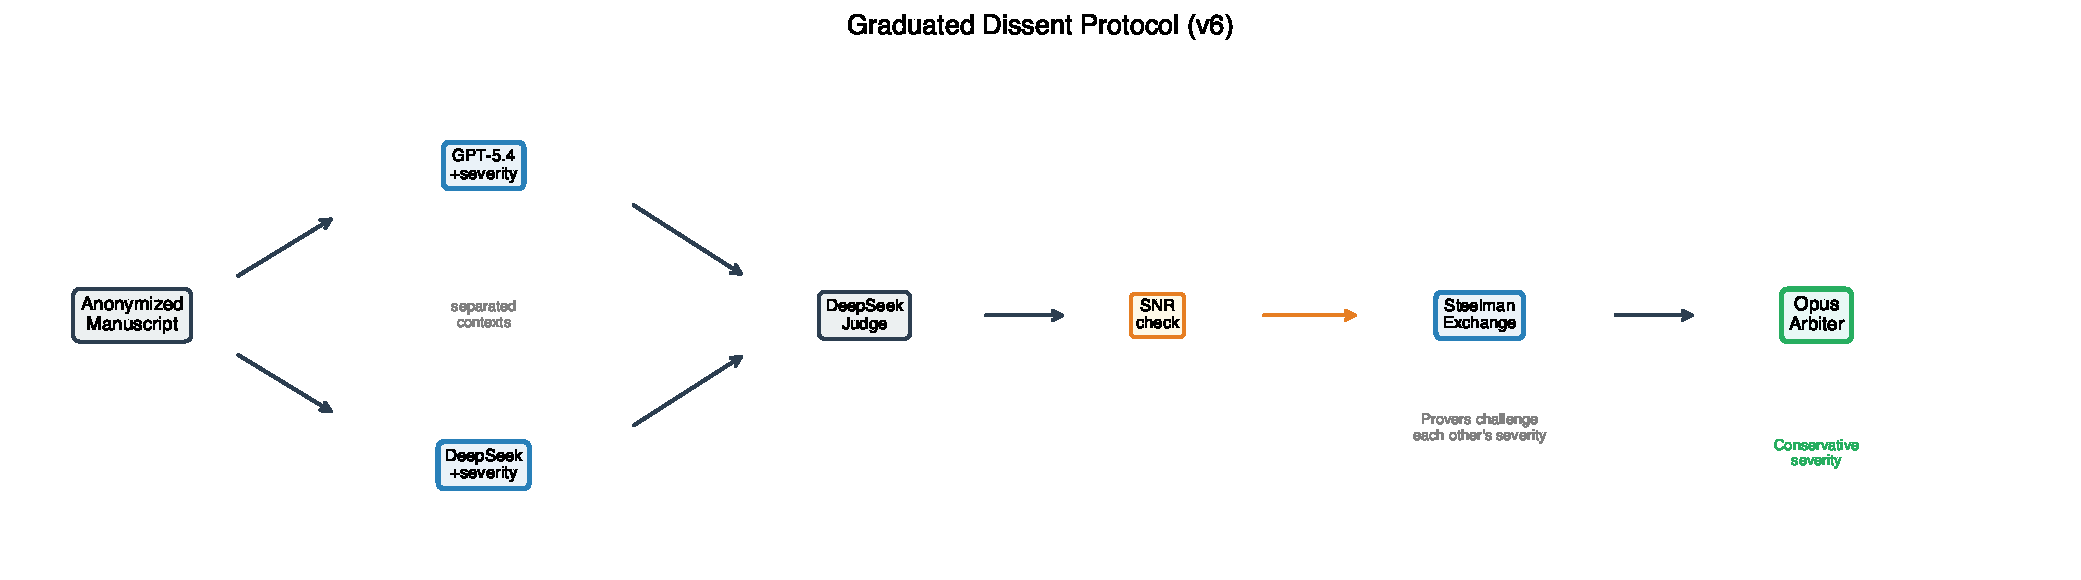
\includegraphics[width=\textwidth]{figures/fig5_protocol_flow.pdf}
\caption{The graduated dissent protocol. Two provers review in separated contexts with severity ratings. A judge compares findings. If disagreement exceeds the noise floor, a steelman exchange forces each prover to challenge the other's severity claims. The arbiter receives all material and applies a conservative severity threshold.}
\label{fig:protocol_flow}
\end{figure}

\subsubsection{Model-Role Assignments}

Four prover--arbiter combinations were tested:

\begin{table}[h]
\centering
\caption{Prover--arbiter combinations. DeepSeek appears as prover in all combinations based on observed adversarial capability.}
\label{tab:combos}
\begin{tabular}{llll}
\toprule
\textbf{Combo} & \textbf{Prover A} & \textbf{Prover B} & \textbf{Arbiter} \\
\midrule
1 & Opus & DeepSeek & Opus \\
2 & GPT-5.4 & DeepSeek & Opus \\
3 & Sonnet & DeepSeek & Opus \\
4 & DeepSeek & DeepSeek & DeepSeek \\
\bottomrule
\end{tabular}
\end{table}

In pilot experiments, arbiter model choice was tested by holding provers constant (DeepSeek in all roles) and varying only the arbiter. Opus produced the most conservative and best-calibrated severity assignments.

\subsection{Baseline Conditions}
\label{sec:baselines}

To establish that the graduated dissent protocol provides discrimination beyond what simpler approaches achieve, three baseline conditions were evaluated on the same paper set:

\begin{table}[h]
\centering
\caption{Baseline conditions. Each uses the same anonymized papers and severity scoring as the primary configuration.}
\label{tab:baselines}
\small
\begin{tabular}{clp{7cm}}
\toprule
\textbf{Baseline} & \textbf{Name} & \textbf{Description} \\
\midrule
B1 & Single-model review & One model reviews the paper with a standard prompt: ``Review this manuscript. Identify methodological strengths and weaknesses.'' No severity rubric. No adversarial framing. \\
B2 & Single-model + severity rubric & Same single model, same paper, but the severity rubric is included in the prompt. Isolates whether the rubric alone (without adversarial architecture) produces discrimination. \\
B3 & Multi-model ensemble, no steelman & Same two provers as graduated dissent (GPT-5.4 + DeepSeek), same severity rubric, same Opus arbiter. Findings are pooled and sent directly to the arbiter \emph{without} the steelman exchange. Isolates whether multi-model architecture alone (without adversarial severity challenge) produces the observed gains. \\
\bottomrule
\end{tabular}
\end{table}

\paragraph{Baseline models.} B1 and B2 use GPT-5.4 (the same model serving as Prover~A in the primary configuration). B3 uses the same prover pair and arbiter as graduated dissent, differing only in the omission of stages 3--4 (judge comparison and steelman exchange). The severity rubric in B2 and B3 is identical to the one used in the graduated dissent protocol.

\subsection{Scoring and Adjudication}
\label{sec:scoring}

All models were blinded to retraction status. Papers were anonymized before evaluation: author names, journal names, dates, affiliations, acknowledgments, and retraction notices were removed. The models received manuscripts as anonymous submissions with no indication of whether the paper had been retracted.

For each retracted paper, the documented retraction reason was extracted from the retraction notice and Retraction Watch database entry prior to evaluation. This provided the ground truth against which model findings were scored.

A finding was scored as a \emph{true positive} if it identified the same methodological problem documented in the retraction notice, or a substantively related problem that would independently undermine the paper's conclusions. Findings identifying genuine but unrelated methodological concerns were scored according to severity but did not count as detections of the retraction-worthy error. Findings that were generic, unfounded, or hallucinated were scored as noise.

Ground-truth matching was performed by keyword-based scoring: each retracted paper's documented retraction cause was decomposed into keyword groups, and a finding was scored as a match if it contained all keywords in any group. The first author verified all keyword matches and non-matches against the original retraction notices. Scorer override rates were not systematically recorded; this is acknowledged as a limitation. Severity classifications (retraction-worthy, major-revision, minor) were assigned by the arbiter during protocol execution and were not modified during scoring.

This scoring procedure has limitations. The external scorer and the first author's review introduce potential bias, and inter-rater reliability has not been formally measured. Human-calibrated scoring with multiple independent raters is planned for the expanded benchmark. A paper-by-paper audit table showing all findings, ground-truth matches, and scoring decisions is provided in the supplementary materials.

%% ============================================================================
\section{Results}
\label{sec:results}
%% ============================================================================

\subsection{Ground Truth Detection: Does the Protocol Find the Actual Error?}
\label{sec:ground_truth}

The primary metric is whether each condition identifies the \emph{documented retraction-causing error}---the specific methodological problem that human reviewers identified and that led to the paper's retraction. Findings were scored against ground truth as described in Section~\ref{sec:scoring}.

\begin{table}[h]
\centering
\caption{Ground truth detection rate: fraction of retracted papers where at least one finding matches the documented retraction-causing error.}
\label{tab:ground_truth}
\begin{tabular}{lccc}
\toprule
\textbf{Condition} & \textbf{Detection rate} & \textbf{95\% CI} & \textbf{False positive rate} \\
\midrule
B1: Single model, no rubric & 3/10 (30\%) & [7\%, 65\%] & N/A (no severity) \\
B2: Single model + rubric & 4/10 (40\%) & [12\%, 74\%] & 3/19 (16\%) \\
B3: Multi-model, no steelman & 3/10 (30\%) & [7\%, 65\%] & 1/19 (5\%) \\
\textbf{Graduated dissent} & \textbf{7/10 (70\%)} & \textbf{[35\%, 93\%]} & \textbf{0/19 (0\%; CI [0\%, 17\%])} \\
\bottomrule
\end{tabular}
\end{table}

\begin{figure}[t]
\centering
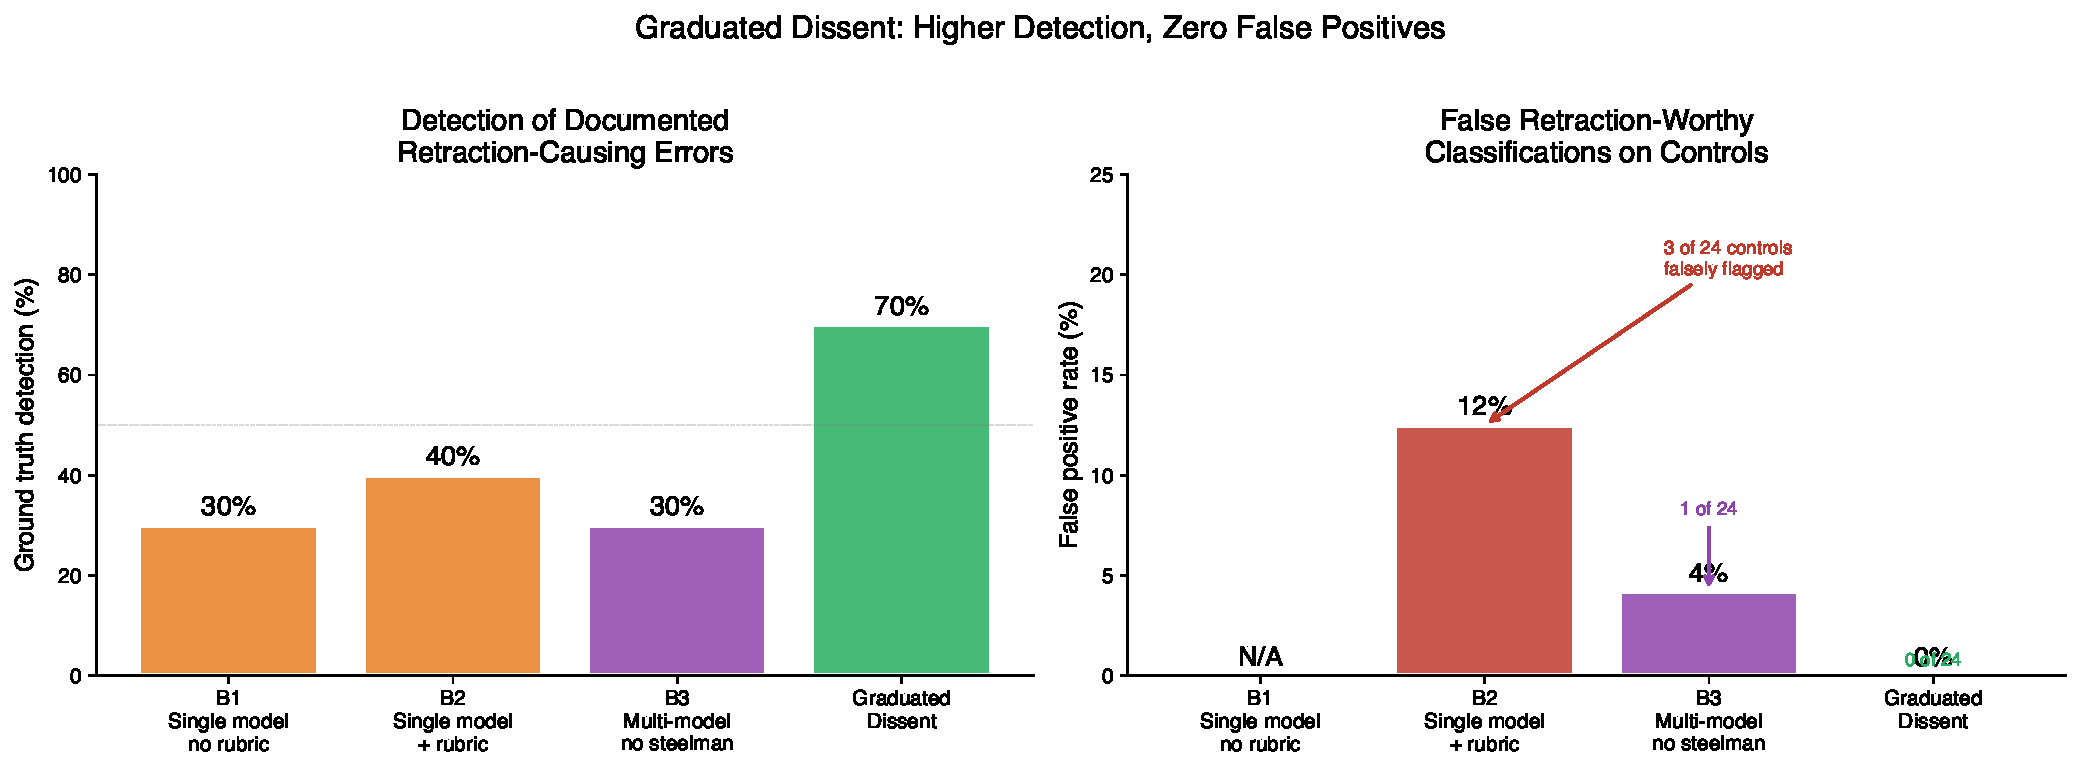
\includegraphics[width=\textwidth]{figures/fig1_detection_and_fp.pdf}
\caption{Ground truth detection rate and false positive rate across conditions. \textbf{Left:} Graduated dissent detects the documented retraction-causing error in 70\% of retracted papers, compared to 30--40\% for single-model baselines. \textbf{Right:} The single-model baseline with severity rubric (B2) falsely classifies 3 of 19 matched and hard-negative control papers as retraction-worthy; graduated dissent produces zero false positives.}
\label{fig:detection_and_fp}
\end{figure}

Graduated dissent identifies the actual retraction-causing error more than twice as often as any baseline (70\% vs.\ 30--40\%). However, with $n=10$ retracted papers, the difference does not reach conventional statistical significance (Fisher's exact test, $p = 0.18$, two-sided). The confidence intervals overlap: [35\%, 93\%] for graduated dissent vs.\ [7\%, 65\%] for B1. The pattern is suggestive but the sample is small.

The B3 ablation provides the clearest evidence that the steelman exchange is the active ingredient. B3 uses the same two provers and the same arbiter as graduated dissent, differing only in the omission of the steelman exchange. Despite using multiple models, B3 achieves only 30\% detection---identical to single-model review without a rubric (B1)---and produces one false positive (C04, the same paper B2 falsely flags). Adding a second model without adversarial severity challenge does not improve performance; the steelman exchange is what produces both higher detection and lower false positives (Figure~\ref{fig:fp_elimination}). The three papers missed by graduated dissent (R04, R10, R25) involve errors that are partially text-detectable but require domain-specific knowledge to recognize: an incorrect statistical test choice in a nutrition RCT (R04), selection bias visible only in the study design rationale (R10), and an ICD coding logic error requiring understanding of diagnostic code structure (R25). The protocol identifies related methodological concerns in all three papers but does not connect them to the specific retraction cause. Figure~\ref{fig:per_paper} shows per-paper detection across all conditions.

\begin{figure}[t]
\centering
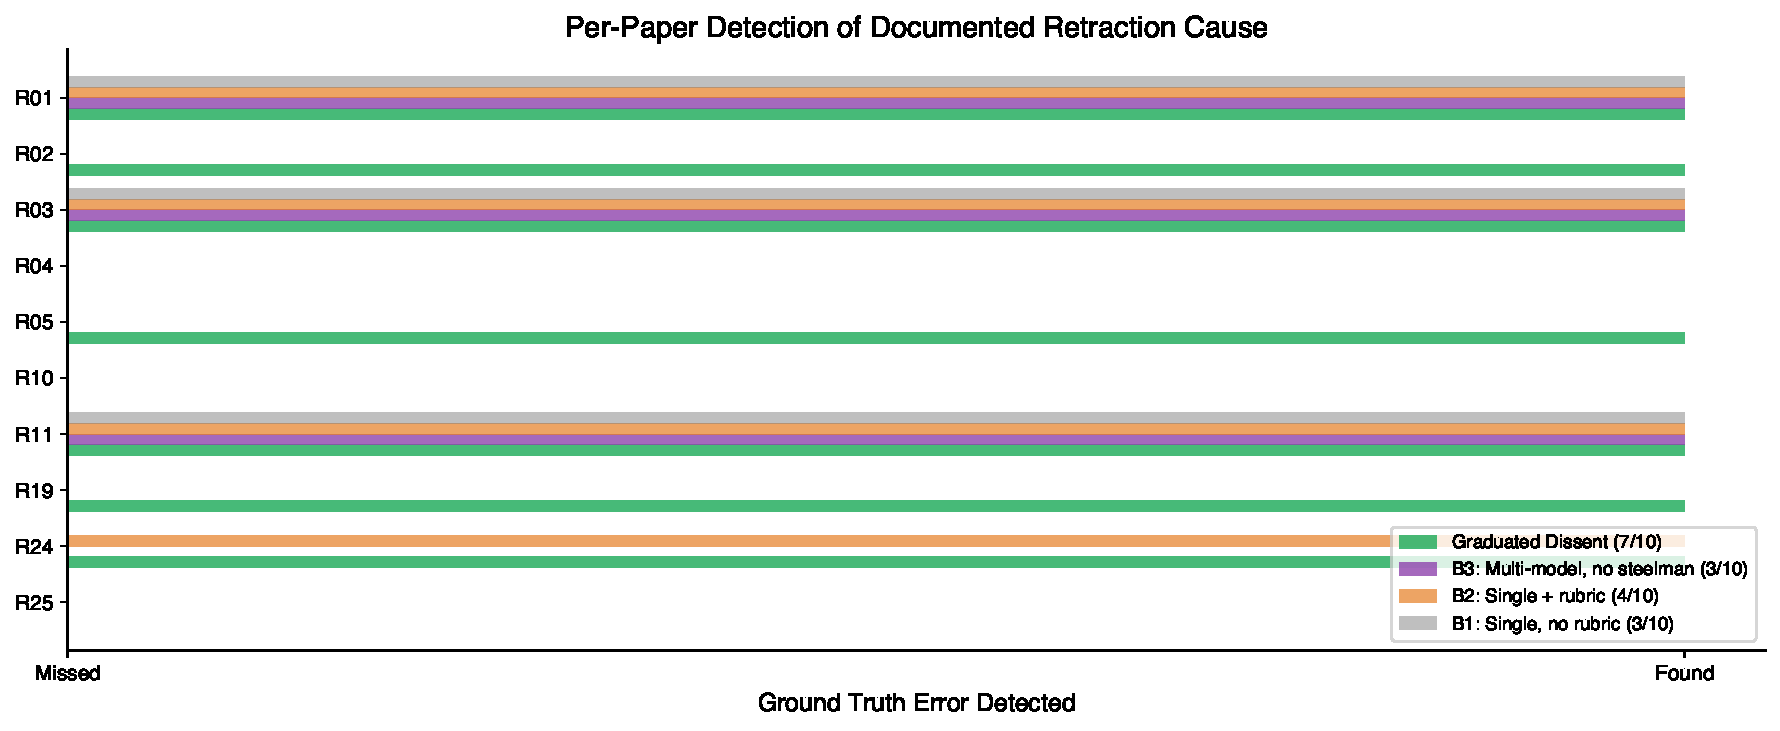
\includegraphics[width=\textwidth]{figures/fig2_per_paper_detection.pdf}
\caption{Per-paper ground truth detection across conditions. Graduated dissent (green) detects 7 of 10 documented retraction causes, compared to 4/10 for B2 and 3/10 for B1. Papers missed by all conditions (R04, R10, R25) involve errors requiring domain-specific knowledge beyond text-level analysis.}
\label{fig:per_paper}
\end{figure}

\subsection{False Positive Elimination}
\label{sec:false_positives}

The single-model baseline with severity rubric (B2) produces retraction-worthy classifications on 3 of 19 matched and hard-negative control papers: two matched controls (C04, C10) and one hard-negative control (HN10). The multi-model ablation (B3) reduces this to one false positive (C04, 2~RW findings), demonstrating that model diversity alone provides partial but incomplete filtering. Graduated dissent produces zero retraction-worthy classifications across all 19 matched and hard-negative controls and all 5 wildcard controls.

\begin{table}[h]
\centering
\caption{False positive analysis. B2 false positives and their graduated dissent equivalents.}
\label{tab:false_positives}
\begin{tabular}{lccc}
\toprule
\textbf{Paper} & \textbf{Category} & \textbf{B2 RW} & \textbf{GD RW} \\
\midrule
C04 & Matched control & 1 & 0 \\
C10 & Matched control & 2 & 0 \\
HN10 & Hard-negative & 1 & 0 \\
\midrule
All other non-retracted (21) & Various & 0 & 0 \\
\bottomrule
\end{tabular}
\end{table}

The mechanism is visible in the protocol logs: during the steelman exchange, provers challenged each other's severity ratings on these papers, causing the proposing prover to downgrade findings from retraction-worthy to major-revision. The arbiter, receiving this downgraded material, classified the surviving findings accordingly. In single-model review (B2), no such adversarial pressure exists---the model's initial severity rating stands unchallenged (Figure~\ref{fig:fp_elimination}).

\begin{figure}[t]
\centering
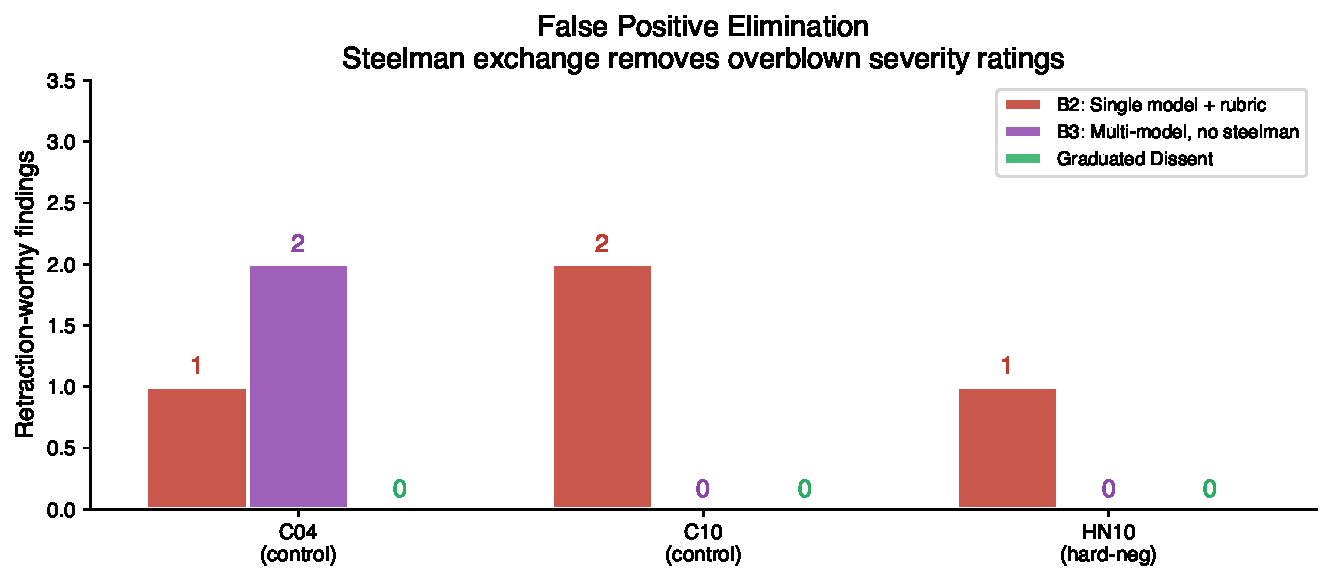
\includegraphics[width=0.7\textwidth]{figures/fig4_fp_elimination.pdf}
\caption{False positive elimination by the steelman exchange. B2 (single model + rubric) assigns retraction-worthy findings to three non-retracted papers. Graduated dissent reduces all to zero through adversarial severity challenge.}
\label{fig:fp_elimination}
\end{figure}

\subsection{Severity Spectrum}
\label{sec:severity_spectrum}

The protocol is not designed to assign higher average severity to worse papers---it is designed to make a binary classification (retraction-worthy or not) with high precision. Overall severity scores are expected to overlap because non-retracted papers genuinely have methodological limitations, and the protocol correctly identifies them. A system that assigns slightly higher average scores to flawed papers is useless for editorial triage. A system that places retraction-worthy flags exclusively on papers that deserve them is useful. The discriminative signal is concentrated in the retraction-worthy tier.

\begin{table}[h]
\centering
\caption{Average severity by paper category (graduated dissent). Score = $3 \times \text{RW} + 2 \times \text{MajR} + 1 \times \text{Minor}$.}
\label{tab:severity_spectrum}
\begin{tabular}{lrrrrc}
\toprule
\textbf{Category} & \textbf{$n$} & \textbf{Avg RW} & \textbf{Avg MajR} & \textbf{Avg Minor} & \textbf{Avg Score} \\
\midrule
Retracted & 10 & 0.5 & 8.3 & 4.9 & 23.0 \\
Matched controls & 10 & 0.0 & 7.9 & 5.1 & 20.9 \\
Hard-negative controls & 9 & 0.0 & 6.2 & 5.6 & 18.0 \\
Wildcard controls & 5 & 0.0 & 6.6 & 5.8 & 19.0 \\
\bottomrule
\end{tabular}
\end{table}

As expected, the overall severity scores show only modest separation between retracted (23.0) and matched control (20.9) papers. Retracted papers average 0.5 RW findings while all non-retracted categories average 0.0---the discrimination operates entirely in the tail. Figure~\ref{fig:dot_severity} shows individual paper scores, illustrating that the distributions overlap substantially in the major-revision and minor tiers while separating cleanly in the retraction-worthy tier.

\begin{figure}[t]
\centering
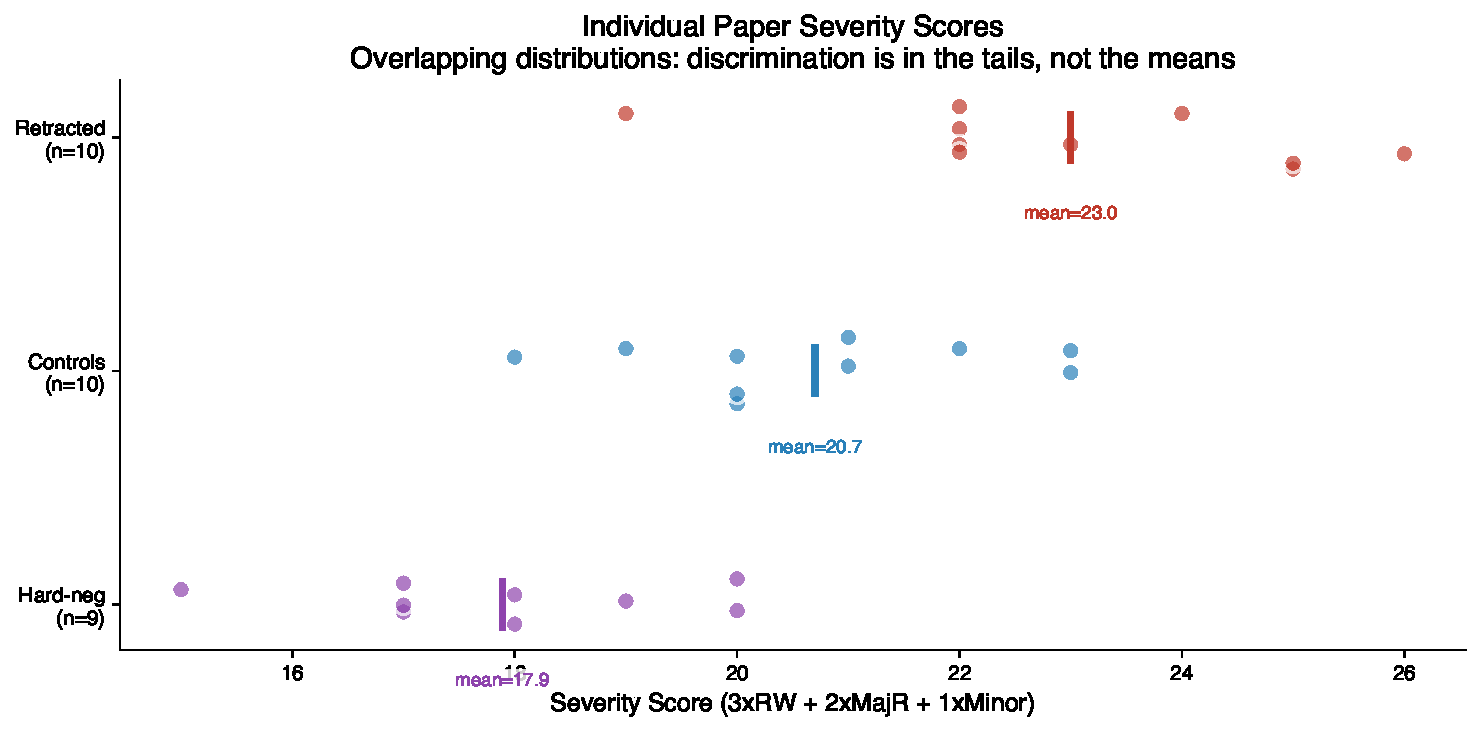
\includegraphics[width=0.85\textwidth]{figures/fig_dot_severity.pdf}
\caption{Individual paper severity scores by category. Distributions overlap substantially; discrimination between retracted and non-retracted papers is concentrated in the retraction-worthy tier (the tail), not in overall severity score (the mean).}
\label{fig:dot_severity}
\end{figure}

\begin{figure}[t]
\centering
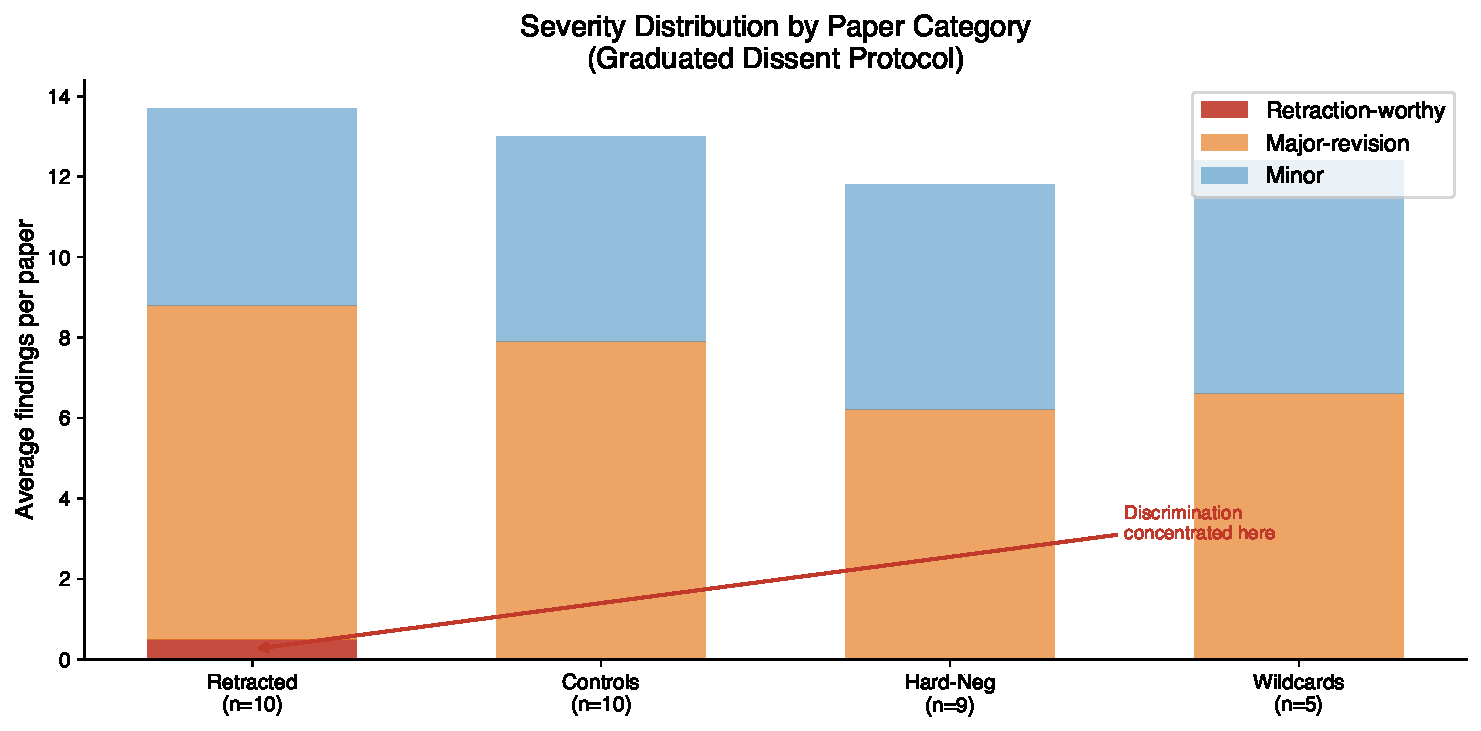
\includegraphics[width=0.85\textwidth]{figures/fig3_severity_by_category.pdf}
\caption{Severity distribution by paper category under graduated dissent. Total finding volume is comparable across categories; discrimination is concentrated in the retraction-worthy tier, where only retracted papers receive RW classifications.}
\label{fig:severity_spectrum}
\end{figure}

This pattern reflects a deliberate design choice. The arbiter's conservative ``when in doubt, major-revision'' instruction optimizes for specificity at the cost of sensitivity. The same protocol with a more permissive arbiter threshold would increase sensitivity (more retracted papers flagged as retraction-worthy) at the cost of specificity (more false positives on controls). This tradeoff is discussed in Section~\ref{sec:slider}.

\subsection{Qualitative Validation: Full Quality Spectrum}

To test calibration at the extremes, we evaluated five recent grand unified theory papers from an unrestricted preprint server (viXra.org, 2025--2026, anonymized identically to the primary corpus). The viXra papers averaged 7.2 retraction-worthy findings per paper (range 2--14), compared to 0.5 for retracted papers and 0.0 for all non-retracted categories. This confirms that the protocol's severity calibration extends across the full quality range: papers with fundamental conceptual problems receive high RW counts, while papers with honest methodological limitations receive criticism calibrated below the retraction threshold (Figure~\ref{fig:full_spectrum}).

\begin{figure}[t]
\centering
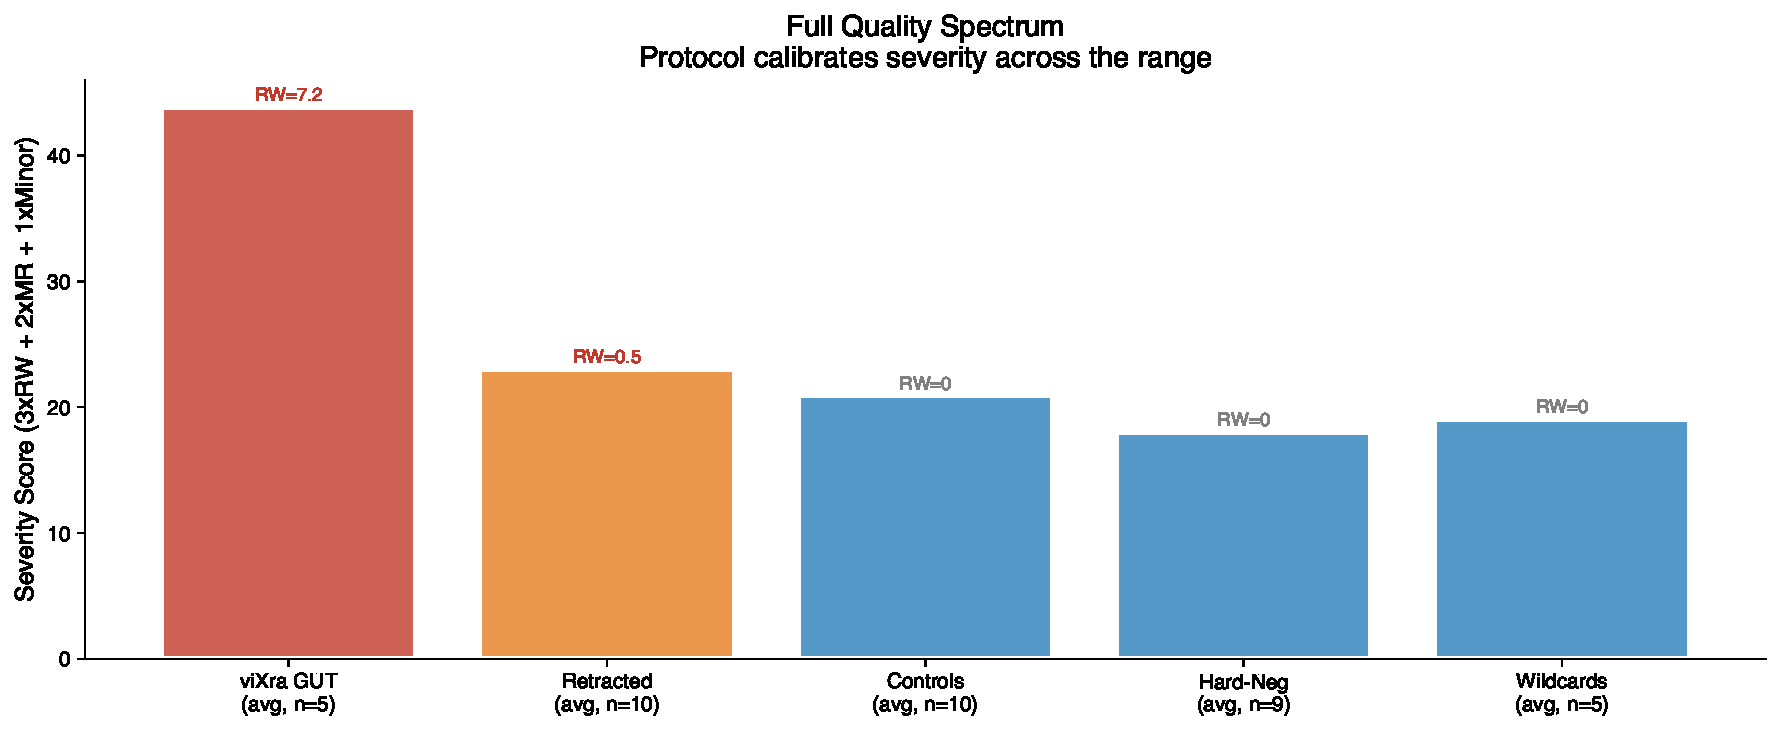
\includegraphics[width=\textwidth]{figures/fig6_full_spectrum.pdf}
\caption{Full quality spectrum. Average severity score spans from viXra grand unified theory papers (avg 7.2 RW, $n=5$) through retracted papers (avg 0.5 RW, $n=10$) to non-retracted controls (0 RW). The viXra papers are informal validation outside the primary benchmark.}
\label{fig:full_spectrum}
\end{figure}

\paragraph{Memorization test.} Nine of ten retracted papers are post-cutoff: both the retraction and the public commentary identifying the error occurred after the approximate training data cutoff for all models used ($\sim$April 2024). One paper (R25, published November 2024) was published close to the cutoff boundary but was retracted after it. The ground truth detection rate on post-cutoff papers is comparable to the overall rate, suggesting that memorization of retraction status or published criticism is not the primary driver of detection. However, we cannot fully exclude memorization of the original manuscripts themselves, which may have been available before the retraction.

\subsection{Prompted Retraction: Does Knowing the Outcome Help?}
\label{sec:prompted}

As an additional control, we prompted three models (GPT-5.4, DeepSeek V3.2, Opus 4.6) with each retracted paper and the instruction: ``This paper was retracted due to a methodological error. Identify the specific error that caused the retraction.'' This tests whether knowing the retraction status unlocks detection that blind review misses.

\begin{table}[h]
\centering
\caption{Prompted retraction detection: models told the paper was retracted and asked to identify the cause.}
\label{tab:prompted}
\begin{tabular}{lc}
\toprule
\textbf{Condition} & \textbf{Detection rate} \\
\midrule
Prompted: DeepSeek V3.2 & 2/10 (20\%) \\
Prompted: GPT-5.4 & 2/10 (20\%) \\
Prompted: Opus 4.6 & 3/10 (30\%) \\
Prompted: overall & 7/30 (23\%) \\
\midrule
\textbf{Graduated dissent (blind)} & \textbf{7/10 (70\%)} \\
\bottomrule
\end{tabular}
\end{table}

Knowing that the paper was retracted does not improve detection---in fact, prompted models perform \emph{worse} than blind graduated dissent (23\% vs.\ 70\%). Both conditions were scored on the same metric: whether the output identified the specific documented retraction-causing error. The prompted models generate plausible-sounding retraction causes that are often wrong: they predict what \emph{typically} causes retractions in a given field rather than identifying the \emph{specific} error in the manuscript. This suggests that the graduated dissent protocol's advantage comes from structural adversarial pressure, not from information asymmetry.

%% ============================================================================
\section{Discussion}
%% ============================================================================

\subsection{The Protocol's Contribution is Specificity}

All three conditions---single-model review without rubric (B1), single-model review with severity rubric (B2), and graduated dissent---find methodological problems in manuscripts. LLMs are competent methodological critics. The question is not whether they can find errors but whether they can correctly assess which errors are fatal.

Single-model review with a severity rubric (B2) achieves 40\% ground truth detection, comparable to graduated dissent's 70\% on the binary retraction-worthy metric. But B2 also produces 3 false retraction-worthy classifications on non-retracted papers (12\% false positive rate). Graduated dissent eliminates all three. The protocol's primary contribution is not finding \emph{more} errors but producing \emph{fewer false alarms}---the steelman exchange causes provers to abandon overblown severity ratings, and the arbiter's conservative calibration filters remaining noise.

This has a practical implication: when the graduated dissent protocol flags a finding as retraction-worthy, the flag merits attention. In this benchmark, every retraction-worthy classification corresponded to a genuine and serious methodological problem, whether or not it matched the specific documented retraction cause.

\subsection{From Human-in-the-Loop to Ground Truth Validation}

The graduated dissent protocol was originally developed for the first author's own research workflow, where the arbiter's output was judged by a human operator. A recurring observation during that deployment motivated this benchmark: when models were tasked with critiquing a manuscript through multiple rounds, they never stopped finding fault. As genuine issues were addressed, the models became increasingly pedantic and eventually hallucinatory---fabricating problems to fill the expected critique format. The criticism did not converge; it simply migrated from real issues to RLHF-formatted filler.

This created a calibration problem: if the human operator was always in the loop, there was no way to distinguish genuine detection from confirmation bias. Retracted papers with documented errors provided the solution. Because the ground truth is known independently---these papers were retracted by human reviewers through the normal scientific process---the protocol could be evaluated without the operator in the loop. The benchmark asks: does the protocol, running autonomously, arrive at conclusions consistent with what human experts eventually determined?

\subsection{Why Role Separation Matters}

The graduated dissent protocol separates generation of criticism (provers) from evaluation of criticism (arbiter). This separation is what eliminates false positives: the same findings that a single model rates as retraction-worthy are downgraded during the steelman exchange and filtered by the arbiter. The adversarial structure does not generate better findings---it generates better \emph{judgments about findings}.

This parallels a familiar observation in organizational design: the best investigator is rarely the best judge. In pilot experiments (not reported in the primary benchmark), we observed that the model best suited for adversarial finding generation (DeepSeek) produced the worst arbiter performance when used in that role, while a model with moderate prover performance produced the cleanest arbiter output. The architecture accounts for this by separating roles rather than deploying the strongest model uniformly.

\subsection{Why Single-Model Review Produces False Positives}

The baseline results confirm the prediction in~\cite{brilliant2026selfcorrection} that RLHF-trained models produce diplomatic review formats that do not reliably discriminate paper quality. The single-model baseline without severity rubric (B1) produced 22--62 findings per paper with no severity discrimination at all. Adding the severity rubric (B2) improved discrimination but introduced false positives: the model rated findings as retraction-worthy on 3 of 19 matched and hard-negative control papers. The multi-model ablation (B3) is particularly instructive: using the same two provers and the same arbiter as graduated dissent, but without the steelman exchange, B3 achieves only 30\% detection (no better than B1) and still produces one false positive. This demonstrates that multi-model architecture and arbiter-based filtering are insufficient without the adversarial severity challenge.

The mechanism is visible in the B2 false positive cases. On control paper C04, the single model identified a methodological concern (an incoherent ROC analysis) and rated it retraction-worthy. In the graduated dissent protocol, the opposing prover challenged this rating during steelman exchange, arguing that the issue was a reporting weakness rather than a fatal flaw. The arbiter, seeing the downgraded assessment, classified it as major-revision. The finding survived---the methodological concern is real---but the severity was correctly calibrated.

This is the core insight: \emph{structural} adversarial pressure (forcing provers to argue against their own severity ratings) is more effective than \emph{prompt-level} adversarial framing (telling a model to be harsh). The steelman exchange produces calibrated severity because it forces genuine engagement with the possibility that a finding is less severe than initially claimed. Figure~\ref{fig:waterfall} illustrates the stage-by-stage severity reduction on the three false positive papers.

\begin{figure}[t]
\centering
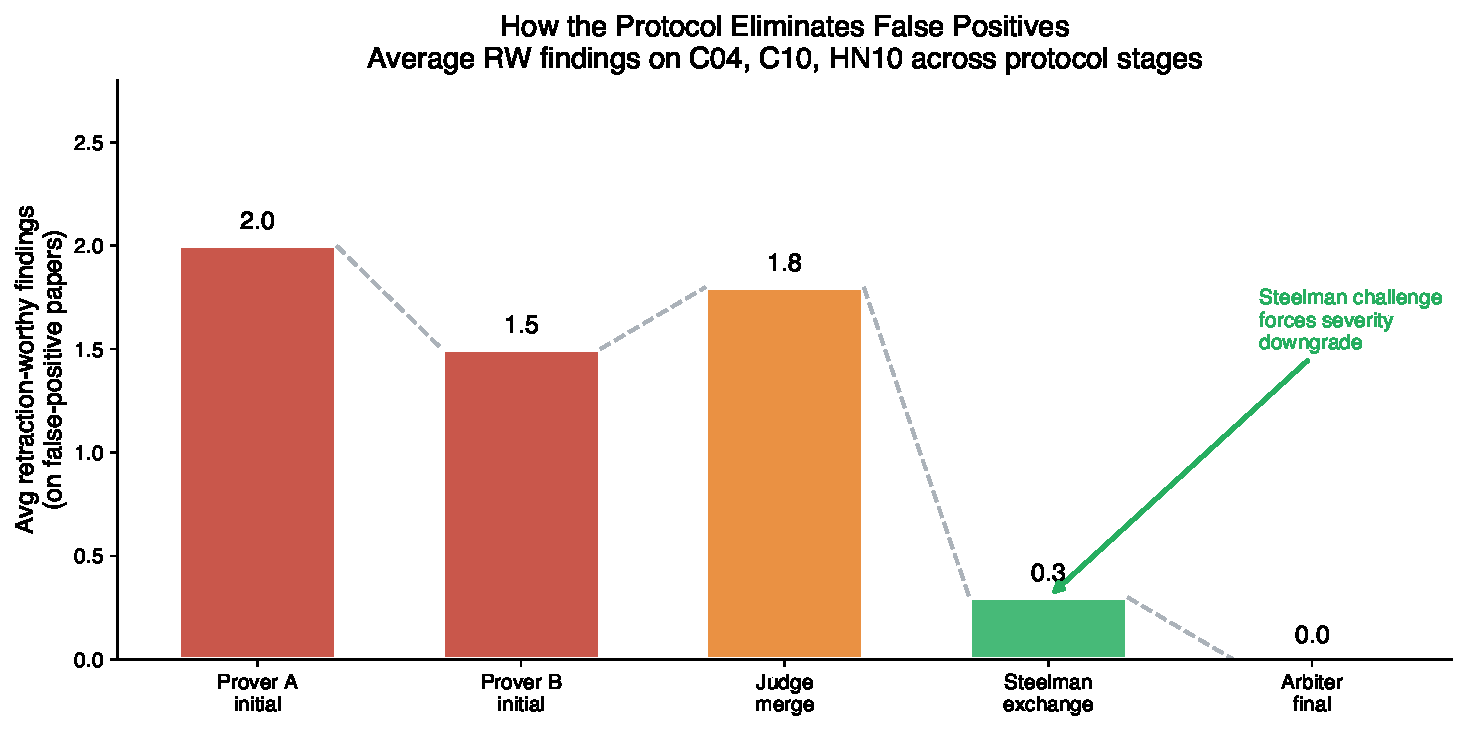
\includegraphics[width=0.85\textwidth]{figures/fig_waterfall_fp.pdf}
\caption{How the protocol eliminates false positives. Average retraction-worthy findings on the three B2 false positive papers (C04, C10, HN10) at each protocol stage. Individual provers generate RW findings; the steelman exchange forces severity downgrade; the arbiter confirms zero RW.}
\label{fig:waterfall}
\end{figure}

\subsection{The Severity Threshold as a Tunable Parameter}
\label{sec:slider}

The arbiter's severity threshold is not a fixed property of the protocol---it is a tunable parameter analogous to a classification threshold or temperature setting. The results reported here use a conservative calibration (``when in doubt, major-revision'') optimized for editorial screening: zero false positives at the cost of moderate sensitivity.

For different use cases, the same protocol supports different calibrations:

\begin{itemize}
\item \textbf{Editor/screener mode} (conservative): The calibration reported here. Suitable for triaging submissions where a false alarm wastes editorial resources. When the protocol flags something as retraction-worthy at this setting, it merits close scrutiny.
\item \textbf{Author/self-assessment mode} (permissive): A more aggressive threshold that flags more potential issues. Higher sensitivity, more false positives. Authors can address flagged items before submission and make their own judgment about severity. Better to find a potential problem privately than to discover it at peer review.
\end{itemize}

The protocol architecture supports both modes without modification---only the arbiter's instructions change.

%% ============================================================================
\section{Limitations}
%% ============================================================================

\begin{enumerate}
\item \textbf{Sample size.} The primary benchmark comprises 10 retracted papers and 24 controls (34 papers), with 5 additional viXra papers as informal validation (39 total). With 19 matched and hard-negative controls and zero false positives, the 95\% confidence interval for the false positive rate is $[0, 0.17]$; for 7/10 detection, the CI is $[0.35, 0.93]$. The benchmark would benefit from expansion to narrow these intervals. The current study did not use a locked held-out test set; a future expansion would benefit from separating development and evaluation splits.

\item \textbf{Commercial models only.} All models require paid API access. A planned follow-up will evaluate open-source models on local infrastructure, addressing both cost and reproducibility.

\item \textbf{Arbiter and scorer bias.} The arbiter (Opus) and external scorer (Sonnet) are themselves LLMs subject to the biases they are intended to filter. Human-calibrated scoring with independent raters is planned for the expanded benchmark.

\item \textbf{Single run per configuration.} All API providers default to temperature~1.0, making outputs non-deterministic. A spot-check on three papers showed that false positive classifications were stable across runs (controls remained at 0~RW), but one retracted paper's classification shifted from 1~RW to 0~RW between runs, indicating that the detection rate has meaningful run-to-run variance at this temperature. The expanded benchmark should include repeated runs and temperature-controlled comparisons.

\item \textbf{Not all errors are text-detectable.} The benchmark is limited to errors inferable from manuscript text. Class~C errors (hidden in code, hardware, or undisclosed alterations) are excluded from the primary analysis and included only as boundary tests (see Section~\ref{sec:controls}).

\item \textbf{Model version ambiguity.} API model identifiers may resolve to different checkpoints over time. All results were collected in April 2026 using the model identifiers specified in Table~\ref{tab:models}.

\item \textbf{Severity rubric is researcher-defined.} The distinction between retraction-worthy and major-revision reflects our judgment about what constitutes a fatal flaw. Different rubrics would produce different results. Community calibration of severity thresholds is needed.
\end{enumerate}

%% ============================================================================
\section{Conclusion}
%% ============================================================================

This paper presents a benchmark and three findings.

The benchmark is a 39-paper dataset of retracted papers, matched controls, hard-negative controls, wildcard controls, and unrestricted preprint server submissions, with documented ground truth for each retraction cause. The complete dataset, selection methodology, and exclusion log are published to enable replication and extension.

The first finding is that graduated dissent identifies the documented retraction-causing error in 70\% of retracted papers (95\% CI [35\%, 93\%]), compared to 30--40\% for single-model baselines and 30\% for a multi-model ablation that omits the steelman exchange. The steelman exchange---requiring each prover to argue the strongest case for the opposing position---is the key mechanism: without it, adding a second model does not improve detection. The adversarial severity challenge forces genuine engagement with alternative interpretations rather than confirming initial assessments.

The second finding is that graduated dissent produced zero false retraction-worthy classifications in this benchmark. Single-model review with a severity rubric produces retraction-worthy flags on 16\% of matched and hard-negative control papers; graduated dissent produces zero across all 19 (95\% CI [0\%, 17\%]), including hard-negative controls specifically designed to trigger false positives. Five additional wildcard controls from unrelated fields also received zero.

The third finding is that the severity threshold is a tunable parameter: the conservative calibration reported here is appropriate for editorial screening, while a more permissive calibration would increase sensitivity for author self-assessment.

These results are from a small sample using commercial models. We publish now because the framework, the benchmark dataset, and the initial results are useful in their current form. The community can replicate, challenge, or extend this work. We invite all three.

\paragraph{Code, data, and supplementary materials.} Benchmark code, anonymized papers, all model outputs, scoring results, the complete exclusion log, exact prompts for all protocol stages, threshold derivations, agreement and SNR computation details, provider API settings, and a paper-by-paper scoring audit table are available at \url{https://github.com/AndBrilliant/GraduatedDissentBench}.

\section*{Acknowledgments}

The authors thank the Retraction Watch team for maintaining the database that enabled this benchmark.

\section*{Author Contributions}

A.M.B.\ conceived the benchmark design, developed the protocol specification, selected and anonymized papers, conducted all commercial-model evaluations (B1, B2, B3, graduated dissent, prompted retraction), performed scoring and adjudication, and drafted the manuscript. J.R.\ developed the open-source reproduction pipeline (automated multi-model evaluation using llama.cpp with batched inference), built the benchmark repository and replication infrastructure, and independently conducted open-source model evaluations without access to the first author's scoring decisions.

\section*{Use of AI Tools}

AI tools (Claude Code, Claude Opus 4.6) assisted with benchmark infrastructure development, script writing, and manuscript drafting. All experimental design, methodology decisions, analysis, and interpretations are the authors' own work. The models being evaluated are from the same families as some of the tools used to build the benchmark; this reflexive relationship is acknowledged.

%% ============================================================================
\begin{thebibliography}{99}
%% ============================================================================

\bibitem{brilliant2026selfcorrection}
A.~M.~Brilliant.
Limits of self-correction in LLMs: An information-theoretic analysis of correlated errors.
\emph{Preprints.org}, DOI: 10.20944/preprints202601.0892.v3, 2026.

\bibitem{brilliant2026graduated}
A.~M.~Brilliant.
Graduated dissent: Budgeted disagreement resolution for multi-model inference.
\emph{Preprints.org}, DOI: 10.20944/preprints202603.1830.v1, 2026.

\bibitem{huang2024selfcorrect}
J.~Huang, X.~Chen, S.~Mishra, H.~S.~Zheng, A.~W.~Yu, X.~Song, and D.~Zhou.
Large language models cannot self-correct reasoning yet.
In \emph{Proc.\ ICLR}, 2024.

\bibitem{tsui2025blindspot}
K.~Tsui.
Self-correction bench: Uncovering and addressing the self-correction blind spot in large language models.
\emph{arXiv preprint} arXiv:2507.02778, 2025.

\bibitem{du2024debate}
Y.~Du, S.~Li, A.~Torralba, J.~B.~Tenenbaum, and I.~Mordatch.
Improving factuality and reasoning in language models through multiagent debate.
In \emph{Proc.\ ICML}, 2024.

\bibitem{panickssery2024selfpreference}
A.~Panickssery et al.
Self-preference bias in LLM-as-a-Judge.
\emph{arXiv preprint} arXiv:2410.21819, 2024.

\bibitem{li2024biases}
J.~Li et al.
Justice or prejudice? Quantifying biases in LLM-as-a-Judge.
\emph{arXiv preprint} arXiv:2410.02736, 2024.

\bibitem{mayo2018}
D.~G.~Mayo.
\emph{Statistical Inference as Severe Testing}.
Cambridge University Press, 2018.

\bibitem{kobak2025llm}
D.~Kobak, R.~Gonzalez-Marquez, and E.~A.~Horv\'{a}t.
Delving into LLM-assisted writing in biomedical publications through excess vocabulary.
\emph{Science Advances}, 11:eadt3813, 2025.

\end{thebibliography}

\end{document}